% Created by tikzDevice version 0.12.6 on 2026-08-03 04:42:02
% !TEX encoding = UTF-8 Unicode
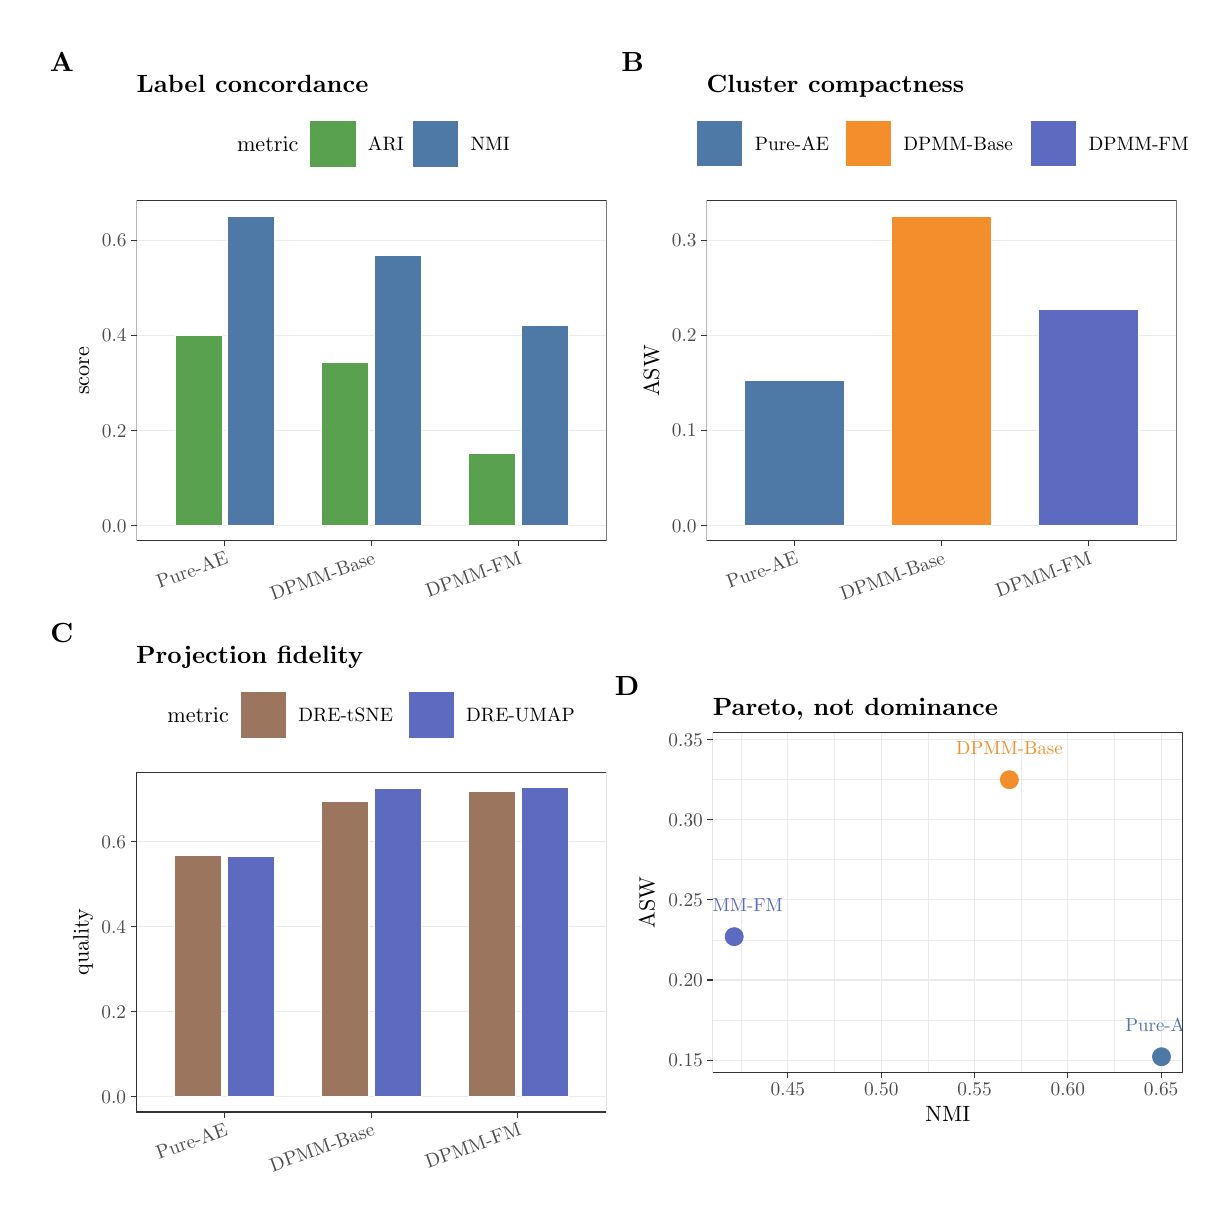
\begin{tikzpicture}[x=1pt,y=1pt]
\definecolor{fillColor}{RGB}{255,255,255}
\path[use as bounding box,fill=fillColor,fill opacity=0.00] (0,0) rectangle (423.43,423.78);
\begin{scope}
\path[clip] (  0.00,  0.00) rectangle (423.43,423.78);
\definecolor{drawColor}{RGB}{255,255,255}
\definecolor{fillColor}{RGB}{255,255,255}

\path[draw=drawColor,line width= 0.6pt,line join=round,line cap=round,fill=fillColor] (  0.00,  0.00) rectangle (423.43,423.78);
\end{scope}
\begin{scope}
\path[clip] (  5.50,211.89) rectangle (211.72,418.28);
\definecolor{drawColor}{RGB}{255,255,255}
\definecolor{fillColor}{RGB}{255,255,255}

\path[draw=drawColor,line width= 0.6pt,line join=round,line cap=round,fill=fillColor] (  5.50,211.89) rectangle (211.72,418.28);
\end{scope}
\begin{scope}
\path[clip] (211.72,211.89) rectangle (417.93,418.28);
\definecolor{drawColor}{RGB}{255,255,255}
\definecolor{fillColor}{RGB}{255,255,255}

\path[draw=drawColor,line width= 0.6pt,line join=round,line cap=round,fill=fillColor] (211.72,211.89) rectangle (417.93,418.28);
\end{scope}
\begin{scope}
\path[clip] (  6.02,212.32) rectangle (211.19,417.85);
\definecolor{drawColor}{RGB}{255,255,255}
\definecolor{fillColor}{RGB}{255,255,255}

\path[draw=drawColor,line width= 0.4pt,line join=round,line cap=round,fill=fillColor] (  6.02,212.32) rectangle (211.19,417.85);
\end{scope}
\begin{scope}
\path[clip] ( 39.36,238.34) rectangle (209.19,361.19);
\definecolor{fillColor}{RGB}{255,255,255}

\path[fill=fillColor] ( 39.36,238.34) rectangle (209.19,361.19);
\definecolor{drawColor}{gray}{0.92}

\path[draw=drawColor,line width= 0.4pt,line join=round] ( 39.36,243.92) --
	(209.19,243.92);

\path[draw=drawColor,line width= 0.4pt,line join=round] ( 39.36,278.28) --
	(209.19,278.28);

\path[draw=drawColor,line width= 0.4pt,line join=round] ( 39.36,312.64) --
	(209.19,312.64);

\path[draw=drawColor,line width= 0.4pt,line join=round] ( 39.36,346.99) --
	(209.19,346.99);
\definecolor{drawColor}{RGB}{255,255,255}
\definecolor{fillColor}{RGB}{78,121,167}

\path[draw=drawColor,line width= 0.2pt,fill=fillColor] (125.34,243.92) rectangle (142.32,341.61);

\path[draw=drawColor,line width= 0.2pt,fill=fillColor] (178.41,243.92) rectangle (195.39,316.28);

\path[draw=drawColor,line width= 0.2pt,fill=fillColor] ( 72.26,243.92) rectangle ( 89.25,355.61);
\definecolor{fillColor}{RGB}{89,161,79}

\path[draw=drawColor,line width= 0.2pt,fill=fillColor] (106.23,243.92) rectangle (123.21,302.79);

\path[draw=drawColor,line width= 0.2pt,fill=fillColor] (159.30,243.92) rectangle (176.29,269.92);

\path[draw=drawColor,line width= 0.2pt,fill=fillColor] ( 53.16,243.92) rectangle ( 70.14,312.69);
\definecolor{drawColor}{gray}{0.20}

\path[draw=drawColor,line width= 0.4pt,line join=round,line cap=round] ( 39.36,238.34) rectangle (209.19,361.19);
\end{scope}
\begin{scope}
\path[clip] (  0.00,  0.00) rectangle (423.43,423.78);
\definecolor{drawColor}{gray}{0.30}

\node[text=drawColor,anchor=base east,inner sep=0pt, outer sep=0pt, scale=  0.70] at ( 35.76,241.51) {0.0};

\node[text=drawColor,anchor=base east,inner sep=0pt, outer sep=0pt, scale=  0.70] at ( 35.76,275.87) {0.2};

\node[text=drawColor,anchor=base east,inner sep=0pt, outer sep=0pt, scale=  0.70] at ( 35.76,310.23) {0.4};

\node[text=drawColor,anchor=base east,inner sep=0pt, outer sep=0pt, scale=  0.70] at ( 35.76,344.58) {0.6};
\end{scope}
\begin{scope}
\path[clip] (  0.00,  0.00) rectangle (423.43,423.78);
\definecolor{drawColor}{gray}{0.20}

\path[draw=drawColor,line width= 0.4pt,line join=round] ( 37.36,243.92) --
	( 39.36,243.92);

\path[draw=drawColor,line width= 0.4pt,line join=round] ( 37.36,278.28) --
	( 39.36,278.28);

\path[draw=drawColor,line width= 0.4pt,line join=round] ( 37.36,312.64) --
	( 39.36,312.64);

\path[draw=drawColor,line width= 0.4pt,line join=round] ( 37.36,346.99) --
	( 39.36,346.99);
\end{scope}
\begin{scope}
\path[clip] (  0.00,  0.00) rectangle (423.43,423.78);
\definecolor{drawColor}{gray}{0.20}

\path[draw=drawColor,line width= 0.4pt,line join=round] ( 71.20,236.34) --
	( 71.20,238.34);

\path[draw=drawColor,line width= 0.4pt,line join=round] (124.28,236.34) --
	(124.28,238.34);

\path[draw=drawColor,line width= 0.4pt,line join=round] (177.35,236.34) --
	(177.35,238.34);
\end{scope}
\begin{scope}
\path[clip] (  0.00,  0.00) rectangle (423.43,423.78);
\definecolor{drawColor}{gray}{0.30}

\node[text=drawColor,rotate= 20.00,anchor=base east,inner sep=0pt, outer sep=0pt, scale=  0.70] at ( 72.85,230.20) {Pure-AE};

\node[text=drawColor,rotate= 20.00,anchor=base east,inner sep=0pt, outer sep=0pt, scale=  0.70] at (125.92,230.20) {DPMM-Base};

\node[text=drawColor,rotate= 20.00,anchor=base east,inner sep=0pt, outer sep=0pt, scale=  0.70] at (179.00,230.20) {DPMM-FM};
\end{scope}
\begin{scope}
\path[clip] (  0.00,  0.00) rectangle (423.43,423.78);
\definecolor{drawColor}{RGB}{0,0,0}

\node[text=drawColor,rotate= 90.00,anchor=base,inner sep=0pt, outer sep=0pt, scale=  0.80] at ( 22.22,299.76) {score};
\end{scope}
\begin{scope}
\path[clip] (  0.00,  0.00) rectangle (423.43,423.78);
\definecolor{fillColor}{RGB}{255,255,255}

\path[fill=fillColor] ( 71.65,369.19) rectangle (176.90,394.54);
\end{scope}
\begin{scope}
\path[clip] (  0.00,  0.00) rectangle (423.43,423.78);
\definecolor{drawColor}{RGB}{0,0,0}

\node[text=drawColor,anchor=base west,inner sep=0pt, outer sep=0pt, scale=  0.80] at ( 75.65,379.11) {metric};
\end{scope}
\begin{scope}
\path[clip] (  0.00,  0.00) rectangle (423.43,423.78);
\definecolor{fillColor}{RGB}{255,255,255}

\path[fill=fillColor] (101.62,373.19) rectangle (118.97,390.54);
\definecolor{drawColor}{RGB}{255,255,255}
\definecolor{fillColor}{RGB}{89,161,79}

\path[draw=drawColor,line width= 0.2pt,fill=fillColor] (101.91,373.48) rectangle (118.68,390.25);
\end{scope}
\begin{scope}
\path[clip] (  0.00,  0.00) rectangle (423.43,423.78);
\definecolor{fillColor}{RGB}{255,255,255}

\path[fill=fillColor] (138.68,373.19) rectangle (156.03,390.54);
\definecolor{drawColor}{RGB}{255,255,255}
\definecolor{fillColor}{RGB}{78,121,167}

\path[draw=drawColor,line width= 0.2pt,fill=fillColor] (138.97,373.48) rectangle (155.74,390.25);
\end{scope}
\begin{scope}
\path[clip] (  0.00,  0.00) rectangle (423.43,423.78);
\definecolor{drawColor}{RGB}{0,0,0}

\node[text=drawColor,anchor=base west,inner sep=0pt, outer sep=0pt, scale=  0.70] at (122.97,379.46) {ARI};
\end{scope}
\begin{scope}
\path[clip] (  0.00,  0.00) rectangle (423.43,423.78);
\definecolor{drawColor}{RGB}{0,0,0}

\node[text=drawColor,anchor=base west,inner sep=0pt, outer sep=0pt, scale=  0.70] at (160.03,379.46) {NMI};
\end{scope}
\begin{scope}
\path[clip] (  0.00,  0.00) rectangle (423.43,423.78);
\definecolor{drawColor}{RGB}{0,0,0}

\node[text=drawColor,anchor=base west,inner sep=0pt, outer sep=0pt, scale=  0.90] at ( 39.36,400.53) {\bfseries Label concordance};
\end{scope}
\begin{scope}
\path[clip] (  0.00,  0.00) rectangle (423.43,423.78);
\definecolor{drawColor}{RGB}{0,0,0}

\node[text=drawColor,anchor=base,inner sep=0pt, outer sep=0pt, scale=  1.00] at ( 12.37,407.84) {\bfseries A};
\end{scope}
\begin{scope}
\path[clip] (212.49,212.32) rectangle (417.15,417.85);
\definecolor{drawColor}{RGB}{255,255,255}
\definecolor{fillColor}{RGB}{255,255,255}

\path[draw=drawColor,line width= 0.4pt,line join=round,line cap=round,fill=fillColor] (212.49,212.32) rectangle (417.15,417.85);
\end{scope}
\begin{scope}
\path[clip] (245.32,238.34) rectangle (415.15,361.19);
\definecolor{fillColor}{RGB}{255,255,255}

\path[fill=fillColor] (245.32,238.34) rectangle (415.15,361.19);
\definecolor{drawColor}{gray}{0.92}

\path[draw=drawColor,line width= 0.4pt,line join=round] (245.32,243.92) --
	(415.15,243.92);

\path[draw=drawColor,line width= 0.4pt,line join=round] (245.32,278.29) --
	(415.15,278.29);

\path[draw=drawColor,line width= 0.4pt,line join=round] (245.32,312.66) --
	(415.15,312.66);

\path[draw=drawColor,line width= 0.4pt,line join=round] (245.32,347.03) --
	(415.15,347.03);
\definecolor{drawColor}{RGB}{255,255,255}
\definecolor{fillColor}{RGB}{242,142,43}

\path[draw=drawColor,line width= 0.3pt,fill=fillColor] (312.19,243.92) rectangle (348.28,355.61);
\definecolor{fillColor}{RGB}{92,107,192}

\path[draw=drawColor,line width= 0.3pt,fill=fillColor] (365.26,243.92) rectangle (401.35,321.96);
\definecolor{fillColor}{RGB}{78,121,167}

\path[draw=drawColor,line width= 0.3pt,fill=fillColor] (259.12,243.92) rectangle (295.20,296.21);
\definecolor{drawColor}{gray}{0.20}

\path[draw=drawColor,line width= 0.4pt,line join=round,line cap=round] (245.32,238.34) rectangle (415.15,361.19);
\end{scope}
\begin{scope}
\path[clip] (  0.00,  0.00) rectangle (423.43,423.78);
\definecolor{drawColor}{gray}{0.30}

\node[text=drawColor,anchor=base east,inner sep=0pt, outer sep=0pt, scale=  0.70] at (241.72,241.51) {0.0};

\node[text=drawColor,anchor=base east,inner sep=0pt, outer sep=0pt, scale=  0.70] at (241.72,275.88) {0.1};

\node[text=drawColor,anchor=base east,inner sep=0pt, outer sep=0pt, scale=  0.70] at (241.72,310.25) {0.2};

\node[text=drawColor,anchor=base east,inner sep=0pt, outer sep=0pt, scale=  0.70] at (241.72,344.62) {0.3};
\end{scope}
\begin{scope}
\path[clip] (  0.00,  0.00) rectangle (423.43,423.78);
\definecolor{drawColor}{gray}{0.20}

\path[draw=drawColor,line width= 0.4pt,line join=round] (243.32,243.92) --
	(245.32,243.92);

\path[draw=drawColor,line width= 0.4pt,line join=round] (243.32,278.29) --
	(245.32,278.29);

\path[draw=drawColor,line width= 0.4pt,line join=round] (243.32,312.66) --
	(245.32,312.66);

\path[draw=drawColor,line width= 0.4pt,line join=round] (243.32,347.03) --
	(245.32,347.03);
\end{scope}
\begin{scope}
\path[clip] (  0.00,  0.00) rectangle (423.43,423.78);
\definecolor{drawColor}{gray}{0.20}

\path[draw=drawColor,line width= 0.4pt,line join=round] (277.16,236.34) --
	(277.16,238.34);

\path[draw=drawColor,line width= 0.4pt,line join=round] (330.23,236.34) --
	(330.23,238.34);

\path[draw=drawColor,line width= 0.4pt,line join=round] (383.31,236.34) --
	(383.31,238.34);
\end{scope}
\begin{scope}
\path[clip] (  0.00,  0.00) rectangle (423.43,423.78);
\definecolor{drawColor}{gray}{0.30}

\node[text=drawColor,rotate= 20.00,anchor=base east,inner sep=0pt, outer sep=0pt, scale=  0.70] at (278.81,230.20) {Pure-AE};

\node[text=drawColor,rotate= 20.00,anchor=base east,inner sep=0pt, outer sep=0pt, scale=  0.70] at (331.88,230.20) {DPMM-Base};

\node[text=drawColor,rotate= 20.00,anchor=base east,inner sep=0pt, outer sep=0pt, scale=  0.70] at (384.96,230.20) {DPMM-FM};
\end{scope}
\begin{scope}
\path[clip] (  0.00,  0.00) rectangle (423.43,423.78);
\definecolor{drawColor}{RGB}{0,0,0}

\node[text=drawColor,rotate= 90.00,anchor=base,inner sep=0pt, outer sep=0pt, scale=  0.80] at (228.18,299.76) {ASW};
\end{scope}
\begin{scope}
\path[clip] (  0.00,  0.00) rectangle (423.43,423.78);
\definecolor{fillColor}{RGB}{255,255,255}

\path[fill=fillColor] (237.41,369.19) rectangle (423.06,394.54);
\end{scope}
\begin{scope}
\path[clip] (  0.00,  0.00) rectangle (423.43,423.78);
\definecolor{fillColor}{RGB}{255,255,255}

\path[fill=fillColor] (241.41,373.19) rectangle (258.76,390.54);
\definecolor{drawColor}{RGB}{255,255,255}
\definecolor{fillColor}{RGB}{78,121,167}

\path[draw=drawColor,line width= 0.3pt,fill=fillColor] (241.77,373.55) rectangle (258.40,390.18);
\end{scope}
\begin{scope}
\path[clip] (  0.00,  0.00) rectangle (423.43,423.78);
\definecolor{fillColor}{RGB}{255,255,255}

\path[fill=fillColor] (295.07,373.19) rectangle (312.42,390.54);
\definecolor{drawColor}{RGB}{255,255,255}
\definecolor{fillColor}{RGB}{242,142,43}

\path[draw=drawColor,line width= 0.3pt,fill=fillColor] (295.43,373.55) rectangle (312.06,390.18);
\end{scope}
\begin{scope}
\path[clip] (  0.00,  0.00) rectangle (423.43,423.78);
\definecolor{fillColor}{RGB}{255,255,255}

\path[fill=fillColor] (362.00,373.19) rectangle (379.34,390.54);
\definecolor{drawColor}{RGB}{255,255,255}
\definecolor{fillColor}{RGB}{92,107,192}

\path[draw=drawColor,line width= 0.3pt,fill=fillColor] (362.35,373.55) rectangle (378.99,390.18);
\end{scope}
\begin{scope}
\path[clip] (  0.00,  0.00) rectangle (423.43,423.78);
\definecolor{drawColor}{RGB}{0,0,0}

\node[text=drawColor,anchor=base west,inner sep=0pt, outer sep=0pt, scale=  0.70] at (262.76,379.46) {Pure-AE};
\end{scope}
\begin{scope}
\path[clip] (  0.00,  0.00) rectangle (423.43,423.78);
\definecolor{drawColor}{RGB}{0,0,0}

\node[text=drawColor,anchor=base west,inner sep=0pt, outer sep=0pt, scale=  0.70] at (316.42,379.46) {DPMM-Base};
\end{scope}
\begin{scope}
\path[clip] (  0.00,  0.00) rectangle (423.43,423.78);
\definecolor{drawColor}{RGB}{0,0,0}

\node[text=drawColor,anchor=base west,inner sep=0pt, outer sep=0pt, scale=  0.70] at (383.34,379.46) {DPMM-FM};
\end{scope}
\begin{scope}
\path[clip] (  0.00,  0.00) rectangle (423.43,423.78);
\definecolor{drawColor}{RGB}{0,0,0}

\node[text=drawColor,anchor=base west,inner sep=0pt, outer sep=0pt, scale=  0.90] at (245.32,400.53) {\bfseries Cluster compactness};
\end{scope}
\begin{scope}
\path[clip] (  0.00,  0.00) rectangle (423.43,423.78);
\definecolor{drawColor}{RGB}{0,0,0}

\node[text=drawColor,anchor=base,inner sep=0pt, outer sep=0pt, scale=  1.00] at (218.58,407.84) {\bfseries B};
\end{scope}
\begin{scope}
\path[clip] (  5.50,  5.50) rectangle (211.72,211.89);
\definecolor{drawColor}{RGB}{255,255,255}
\definecolor{fillColor}{RGB}{255,255,255}

\path[draw=drawColor,line width= 0.6pt,line join=round,line cap=round,fill=fillColor] (  5.50,  5.50) rectangle (211.72,211.89);
\end{scope}
\begin{scope}
\path[clip] (211.72,  5.50) rectangle (417.93,211.89);
\definecolor{drawColor}{RGB}{255,255,255}
\definecolor{fillColor}{RGB}{255,255,255}

\path[draw=drawColor,line width= 0.6pt,line join=round,line cap=round,fill=fillColor] (211.72,  5.50) rectangle (417.93,211.89);
\end{scope}
\begin{scope}
\path[clip] (  6.22,  5.93) rectangle (211.00,211.46);
\definecolor{drawColor}{RGB}{255,255,255}
\definecolor{fillColor}{RGB}{255,255,255}

\path[draw=drawColor,line width= 0.4pt,line join=round,line cap=round,fill=fillColor] (  6.22,  5.93) rectangle (211.00,211.46);
\end{scope}
\begin{scope}
\path[clip] ( 39.16, 31.95) rectangle (209.00,154.81);
\definecolor{fillColor}{RGB}{255,255,255}

\path[fill=fillColor] ( 39.16, 31.95) rectangle (209.00,154.81);
\definecolor{drawColor}{gray}{0.92}

\path[draw=drawColor,line width= 0.4pt,line join=round] ( 39.16, 37.53) --
	(209.00, 37.53);

\path[draw=drawColor,line width= 0.4pt,line join=round] ( 39.16, 68.21) --
	(209.00, 68.21);

\path[draw=drawColor,line width= 0.4pt,line join=round] ( 39.16, 98.89) --
	(209.00, 98.89);

\path[draw=drawColor,line width= 0.4pt,line join=round] ( 39.16,129.57) --
	(209.00,129.57);
\definecolor{drawColor}{RGB}{255,255,255}
\definecolor{fillColor}{RGB}{92,107,192}

\path[draw=drawColor,line width= 0.2pt,fill=fillColor] (125.14, 37.53) rectangle (142.13,148.88);

\path[draw=drawColor,line width= 0.2pt,fill=fillColor] (178.22, 37.53) rectangle (195.20,149.22);

\path[draw=drawColor,line width= 0.2pt,fill=fillColor] ( 72.07, 37.53) rectangle ( 89.05,124.23);
\definecolor{fillColor}{RGB}{156,117,95}

\path[draw=drawColor,line width= 0.2pt,fill=fillColor] (106.04, 37.53) rectangle (123.02,144.29);

\path[draw=drawColor,line width= 0.2pt,fill=fillColor] (159.11, 37.53) rectangle (176.09,147.68);

\path[draw=drawColor,line width= 0.2pt,fill=fillColor] ( 52.96, 37.53) rectangle ( 69.95,124.76);
\definecolor{drawColor}{gray}{0.20}

\path[draw=drawColor,line width= 0.4pt,line join=round,line cap=round] ( 39.16, 31.95) rectangle (209.00,154.81);
\end{scope}
\begin{scope}
\path[clip] (  0.00,  0.00) rectangle (423.43,423.78);
\definecolor{drawColor}{gray}{0.30}

\node[text=drawColor,anchor=base east,inner sep=0pt, outer sep=0pt, scale=  0.70] at ( 35.56, 35.12) {0.0};

\node[text=drawColor,anchor=base east,inner sep=0pt, outer sep=0pt, scale=  0.70] at ( 35.56, 65.80) {0.2};

\node[text=drawColor,anchor=base east,inner sep=0pt, outer sep=0pt, scale=  0.70] at ( 35.56, 96.48) {0.4};

\node[text=drawColor,anchor=base east,inner sep=0pt, outer sep=0pt, scale=  0.70] at ( 35.56,127.15) {0.6};
\end{scope}
\begin{scope}
\path[clip] (  0.00,  0.00) rectangle (423.43,423.78);
\definecolor{drawColor}{gray}{0.20}

\path[draw=drawColor,line width= 0.4pt,line join=round] ( 37.16, 37.53) --
	( 39.16, 37.53);

\path[draw=drawColor,line width= 0.4pt,line join=round] ( 37.16, 68.21) --
	( 39.16, 68.21);

\path[draw=drawColor,line width= 0.4pt,line join=round] ( 37.16, 98.89) --
	( 39.16, 98.89);

\path[draw=drawColor,line width= 0.4pt,line join=round] ( 37.16,129.57) --
	( 39.16,129.57);
\end{scope}
\begin{scope}
\path[clip] (  0.00,  0.00) rectangle (423.43,423.78);
\definecolor{drawColor}{gray}{0.20}

\path[draw=drawColor,line width= 0.4pt,line join=round] ( 71.01, 29.95) --
	( 71.01, 31.95);

\path[draw=drawColor,line width= 0.4pt,line join=round] (124.08, 29.95) --
	(124.08, 31.95);

\path[draw=drawColor,line width= 0.4pt,line join=round] (177.15, 29.95) --
	(177.15, 31.95);
\end{scope}
\begin{scope}
\path[clip] (  0.00,  0.00) rectangle (423.43,423.78);
\definecolor{drawColor}{gray}{0.30}

\node[text=drawColor,rotate= 20.00,anchor=base east,inner sep=0pt, outer sep=0pt, scale=  0.70] at ( 72.66, 23.82) {Pure-AE};

\node[text=drawColor,rotate= 20.00,anchor=base east,inner sep=0pt, outer sep=0pt, scale=  0.70] at (125.73, 23.82) {DPMM-Base};

\node[text=drawColor,rotate= 20.00,anchor=base east,inner sep=0pt, outer sep=0pt, scale=  0.70] at (178.80, 23.82) {DPMM-FM};
\end{scope}
\begin{scope}
\path[clip] (  0.00,  0.00) rectangle (423.43,423.78);
\definecolor{drawColor}{RGB}{0,0,0}

\node[text=drawColor,rotate= 90.00,anchor=base,inner sep=0pt, outer sep=0pt, scale=  0.80] at ( 22.03, 93.38) {quality};
\end{scope}
\begin{scope}
\path[clip] (  0.00,  0.00) rectangle (423.43,423.78);
\definecolor{fillColor}{RGB}{255,255,255}

\path[fill=fillColor] ( 46.46,162.81) rectangle (201.70,188.15);
\end{scope}
\begin{scope}
\path[clip] (  0.00,  0.00) rectangle (423.43,423.78);
\definecolor{drawColor}{RGB}{0,0,0}

\node[text=drawColor,anchor=base west,inner sep=0pt, outer sep=0pt, scale=  0.80] at ( 50.46,172.72) {metric};
\end{scope}
\begin{scope}
\path[clip] (  0.00,  0.00) rectangle (423.43,423.78);
\definecolor{fillColor}{RGB}{255,255,255}

\path[fill=fillColor] ( 76.44,166.81) rectangle ( 93.79,184.15);
\definecolor{drawColor}{RGB}{255,255,255}
\definecolor{fillColor}{RGB}{156,117,95}

\path[draw=drawColor,line width= 0.2pt,fill=fillColor] ( 76.72,167.09) rectangle ( 93.50,183.87);
\end{scope}
\begin{scope}
\path[clip] (  0.00,  0.00) rectangle (423.43,423.78);
\definecolor{fillColor}{RGB}{255,255,255}

\path[fill=fillColor] (137.12,166.81) rectangle (154.46,184.15);
\definecolor{drawColor}{RGB}{255,255,255}
\definecolor{fillColor}{RGB}{92,107,192}

\path[draw=drawColor,line width= 0.2pt,fill=fillColor] (137.40,167.09) rectangle (154.18,183.87);
\end{scope}
\begin{scope}
\path[clip] (  0.00,  0.00) rectangle (423.43,423.78);
\definecolor{drawColor}{RGB}{0,0,0}

\node[text=drawColor,anchor=base west,inner sep=0pt, outer sep=0pt, scale=  0.70] at ( 97.79,173.07) {DRE-tSNE};
\end{scope}
\begin{scope}
\path[clip] (  0.00,  0.00) rectangle (423.43,423.78);
\definecolor{drawColor}{RGB}{0,0,0}

\node[text=drawColor,anchor=base west,inner sep=0pt, outer sep=0pt, scale=  0.70] at (158.46,173.07) {DRE-UMAP};
\end{scope}
\begin{scope}
\path[clip] (  0.00,  0.00) rectangle (423.43,423.78);
\definecolor{drawColor}{RGB}{0,0,0}

\node[text=drawColor,anchor=base west,inner sep=0pt, outer sep=0pt, scale=  0.90] at ( 39.16,194.14) {\bfseries Projection fidelity};
\end{scope}
\begin{scope}
\path[clip] (  0.00,  0.00) rectangle (423.43,423.78);
\definecolor{drawColor}{RGB}{0,0,0}

\node[text=drawColor,anchor=base,inner sep=0pt, outer sep=0pt, scale=  1.00] at ( 12.37,201.45) {\bfseries C};
\end{scope}
\begin{scope}
\path[clip] (210.22, 24.88) rectangle (419.42,192.51);
\definecolor{drawColor}{RGB}{255,255,255}
\definecolor{fillColor}{RGB}{255,255,255}

\path[draw=drawColor,line width= 0.4pt,line join=round,line cap=round,fill=fillColor] (210.22, 24.88) rectangle (419.42,192.51);
\end{scope}
\begin{scope}
\path[clip] (247.59, 46.34) rectangle (417.42,169.20);
\definecolor{fillColor}{RGB}{255,255,255}

\path[fill=fillColor] (247.59, 46.34) rectangle (417.42,169.20);
\definecolor{drawColor}{gray}{0.92}

\path[draw=drawColor,line width= 0.2pt,line join=round] (247.59, 65.17) --
	(417.42, 65.17);

\path[draw=drawColor,line width= 0.2pt,line join=round] (247.59, 94.14) --
	(417.42, 94.14);

\path[draw=drawColor,line width= 0.2pt,line join=round] (247.59,123.10) --
	(417.42,123.10);

\path[draw=drawColor,line width= 0.2pt,line join=round] (247.59,152.06) --
	(417.42,152.06);

\path[draw=drawColor,line width= 0.2pt,line join=round] (257.86, 46.34) --
	(257.86,169.20);

\path[draw=drawColor,line width= 0.2pt,line join=round] (291.58, 46.34) --
	(291.58,169.20);

\path[draw=drawColor,line width= 0.2pt,line join=round] (325.30, 46.34) --
	(325.30,169.20);

\path[draw=drawColor,line width= 0.2pt,line join=round] (359.02, 46.34) --
	(359.02,169.20);

\path[draw=drawColor,line width= 0.2pt,line join=round] (392.74, 46.34) --
	(392.74,169.20);

\path[draw=drawColor,line width= 0.4pt,line join=round] (247.59, 50.69) --
	(417.42, 50.69);

\path[draw=drawColor,line width= 0.4pt,line join=round] (247.59, 79.66) --
	(417.42, 79.66);

\path[draw=drawColor,line width= 0.4pt,line join=round] (247.59,108.62) --
	(417.42,108.62);

\path[draw=drawColor,line width= 0.4pt,line join=round] (247.59,137.58) --
	(417.42,137.58);

\path[draw=drawColor,line width= 0.4pt,line join=round] (247.59,166.54) --
	(417.42,166.54);

\path[draw=drawColor,line width= 0.4pt,line join=round] (274.72, 46.34) --
	(274.72,169.20);

\path[draw=drawColor,line width= 0.4pt,line join=round] (308.44, 46.34) --
	(308.44,169.20);

\path[draw=drawColor,line width= 0.4pt,line join=round] (342.16, 46.34) --
	(342.16,169.20);

\path[draw=drawColor,line width= 0.4pt,line join=round] (375.88, 46.34) --
	(375.88,169.20);

\path[draw=drawColor,line width= 0.4pt,line join=round] (409.60, 46.34) --
	(409.60,169.20);
\definecolor{drawColor}{RGB}{242,142,43}
\definecolor{fillColor}{RGB}{242,142,43}

\path[draw=drawColor,line width= 0.3pt,line join=round,line cap=round,fill=fillColor] (354.74,152.03) circle (  3.26);
\definecolor{drawColor}{RGB}{92,107,192}
\definecolor{fillColor}{RGB}{92,107,192}

\path[draw=drawColor,line width= 0.3pt,line join=round,line cap=round,fill=fillColor] (255.31, 95.32) circle (  3.26);
\definecolor{drawColor}{RGB}{78,121,167}
\definecolor{fillColor}{RGB}{78,121,167}

\path[draw=drawColor,line width= 0.3pt,line join=round,line cap=round,fill=fillColor] (409.70, 51.93) circle (  3.26);
\definecolor{drawColor}{RGB}{242,142,43}

\node[text=drawColor,anchor=base,inner sep=0pt, outer sep=0pt, scale=  0.68] at (354.74,161.27) {DPMM-Base};
\definecolor{drawColor}{RGB}{92,107,192}

\node[text=drawColor,anchor=base,inner sep=0pt, outer sep=0pt, scale=  0.68] at (255.31,104.56) {DPMM-FM};
\definecolor{drawColor}{RGB}{78,121,167}

\node[text=drawColor,anchor=base,inner sep=0pt, outer sep=0pt, scale=  0.68] at (409.70, 61.16) {Pure-AE};
\definecolor{drawColor}{gray}{0.20}

\path[draw=drawColor,line width= 0.4pt,line join=round,line cap=round] (247.59, 46.34) rectangle (417.42,169.20);
\end{scope}
\begin{scope}
\path[clip] (  0.00,  0.00) rectangle (423.43,423.78);
\definecolor{drawColor}{gray}{0.30}

\node[text=drawColor,anchor=base east,inner sep=0pt, outer sep=0pt, scale=  0.70] at (243.99, 48.28) {0.15};

\node[text=drawColor,anchor=base east,inner sep=0pt, outer sep=0pt, scale=  0.70] at (243.99, 77.24) {0.20};

\node[text=drawColor,anchor=base east,inner sep=0pt, outer sep=0pt, scale=  0.70] at (243.99,106.21) {0.25};

\node[text=drawColor,anchor=base east,inner sep=0pt, outer sep=0pt, scale=  0.70] at (243.99,135.17) {0.30};

\node[text=drawColor,anchor=base east,inner sep=0pt, outer sep=0pt, scale=  0.70] at (243.99,164.13) {0.35};
\end{scope}
\begin{scope}
\path[clip] (  0.00,  0.00) rectangle (423.43,423.78);
\definecolor{drawColor}{gray}{0.20}

\path[draw=drawColor,line width= 0.4pt,line join=round] (245.59, 50.69) --
	(247.59, 50.69);

\path[draw=drawColor,line width= 0.4pt,line join=round] (245.59, 79.66) --
	(247.59, 79.66);

\path[draw=drawColor,line width= 0.4pt,line join=round] (245.59,108.62) --
	(247.59,108.62);

\path[draw=drawColor,line width= 0.4pt,line join=round] (245.59,137.58) --
	(247.59,137.58);

\path[draw=drawColor,line width= 0.4pt,line join=round] (245.59,166.54) --
	(247.59,166.54);
\end{scope}
\begin{scope}
\path[clip] (  0.00,  0.00) rectangle (423.43,423.78);
\definecolor{drawColor}{gray}{0.20}

\path[draw=drawColor,line width= 0.4pt,line join=round] (274.72, 44.34) --
	(274.72, 46.34);

\path[draw=drawColor,line width= 0.4pt,line join=round] (308.44, 44.34) --
	(308.44, 46.34);

\path[draw=drawColor,line width= 0.4pt,line join=round] (342.16, 44.34) --
	(342.16, 46.34);

\path[draw=drawColor,line width= 0.4pt,line join=round] (375.88, 44.34) --
	(375.88, 46.34);

\path[draw=drawColor,line width= 0.4pt,line join=round] (409.60, 44.34) --
	(409.60, 46.34);
\end{scope}
\begin{scope}
\path[clip] (  0.00,  0.00) rectangle (423.43,423.78);
\definecolor{drawColor}{gray}{0.30}

\node[text=drawColor,anchor=base,inner sep=0pt, outer sep=0pt, scale=  0.70] at (274.72, 37.92) {0.45};

\node[text=drawColor,anchor=base,inner sep=0pt, outer sep=0pt, scale=  0.70] at (308.44, 37.92) {0.50};

\node[text=drawColor,anchor=base,inner sep=0pt, outer sep=0pt, scale=  0.70] at (342.16, 37.92) {0.55};

\node[text=drawColor,anchor=base,inner sep=0pt, outer sep=0pt, scale=  0.70] at (375.88, 37.92) {0.60};

\node[text=drawColor,anchor=base,inner sep=0pt, outer sep=0pt, scale=  0.70] at (409.60, 37.92) {0.65};
\end{scope}
\begin{scope}
\path[clip] (  0.00,  0.00) rectangle (423.43,423.78);
\definecolor{drawColor}{RGB}{0,0,0}

\node[text=drawColor,anchor=base,inner sep=0pt, outer sep=0pt, scale=  0.80] at (332.51, 28.64) {NMI};
\end{scope}
\begin{scope}
\path[clip] (  0.00,  0.00) rectangle (423.43,423.78);
\definecolor{drawColor}{RGB}{0,0,0}

\node[text=drawColor,rotate= 90.00,anchor=base,inner sep=0pt, outer sep=0pt, scale=  0.80] at (226.55,107.77) {ASW};
\end{scope}
\begin{scope}
\path[clip] (  0.00,  0.00) rectangle (423.43,423.78);
\definecolor{drawColor}{RGB}{0,0,0}

\node[text=drawColor,anchor=base west,inner sep=0pt, outer sep=0pt, scale=  0.90] at (247.59,175.19) {\bfseries Pareto, not dominance};
\end{scope}
\begin{scope}
\path[clip] (  0.00,  0.00) rectangle (423.43,423.78);
\definecolor{drawColor}{RGB}{0,0,0}

\node[text=drawColor,anchor=base,inner sep=0pt, outer sep=0pt, scale=  1.00] at (216.63,182.51) {\bfseries D};
\end{scope}
\end{tikzpicture}
